% Template for Cogsci submission with R Markdown

% Stuff changed from original Markdown PLOS Template
\documentclass[10pt, letterpaper]{article}

\usepackage{cogsci}
\usepackage{pslatex}
\usepackage{float}
\usepackage{caption}

% amsmath package, useful for mathematical formulas
\usepackage{amsmath}

% amssymb package, useful for mathematical symbols
\usepackage{amssymb}

% hyperref package, useful for hyperlinks
\usepackage{hyperref}

% graphicx package, useful for including eps and pdf graphics
% include graphics with the command \includegraphics
\usepackage{graphicx}

% Sweave(-like)
\usepackage{fancyvrb}
\DefineVerbatimEnvironment{Sinput}{Verbatim}{fontshape=sl}
\DefineVerbatimEnvironment{Soutput}{Verbatim}{}
\DefineVerbatimEnvironment{Scode}{Verbatim}{fontshape=sl}
\newenvironment{Schunk}{}{}
\DefineVerbatimEnvironment{Code}{Verbatim}{}
\DefineVerbatimEnvironment{CodeInput}{Verbatim}{fontshape=sl}
\DefineVerbatimEnvironment{CodeOutput}{Verbatim}{}
\newenvironment{CodeChunk}{}{}

% cite package, to clean up citations in the main text. Do not remove.
\usepackage{apacite}

% KM added 1/4/18 to allow control of blind submission


\usepackage{color}

% Use doublespacing - comment out for single spacing
%\usepackage{setspace}
%\doublespacing


% % Text layout
% \topmargin 0.0cm
% \oddsidemargin 0.5cm
% \evensidemargin 0.5cm
% \textwidth 16cm
% \textheight 21cm

\title{Developmental changes in the ability to draw distinctive features of
object categories}


\author{{\large \bf Bria Long (bria@stanford.edu)} \\ Department of Psychology, 450 Serra Mall \\ Stanford, CA 94305 \AND {\large \bf Judith E. Fan (jefan@stanford.edu)} \\Department of Psychology, 450 Serra Mall \\ Stanford, CA 94305 \AND {\large \bf Zixian Chai (zchai14@stanford.edu)} \\Department of Psychology, 450 Serra Mall \\ Stanford, CA 94305 \AND {\large \bf Michael C. Frank (mcfrank@stanford.edu)} \\Department of Psychology, 450 Serra Mall \\ Stanford, CA 94305}

\begin{document}

\maketitle

\begin{abstract}
Include no author information in the initial submission, to facilitate
blind review. The abstract should be one paragraph, indented 1/8 inch on
both sides, in 9\textasciitilde{}point font with single spacing. The
heading `Abstract' should be 10\textasciitilde{}point, bold, centered,
with one line of space below it. This one-paragraph abstract section is
required only for standard six page proceedings papers. Following the
abstract should be a blank line, followed by the header `Keywords' and a
list of descriptive keywords separated by semicolons, all in
9\textasciitilde{}point font, as shown below.

\textbf{Keywords:}
object representations; child development; visual production; deep
neural networks
\end{abstract}

\section{Introduction}\label{introduction}

Children draw prolifically, providing a rich source of potential insight
into their emerging understanding of the world (Kellogg, 1969).
Accordingly, drawings have often been used as a method for probing
developmental change in a wide variety of domains (Karmiloff-Smith,
1990, Fury, Carlson, \& Sroufe (1997), Arden, Trzaskowski, Garfield, \&
Plomin (2014); Piaget, 1929). In particular, drawings have long provided
inspiration for scientists investigating the development of visual
concepts (Minsky \& Papert, 1972). For example, even when drawing from
life, children tend to include features invisible from their vantage
point yet diagnostic of category membership (e.g., a handle on a mug)
(Bremner \& Moore, 1984, Barrett \& Light (1976)). Indeed, several adult
studies suggest that there may be a systematic relationship between our
representations of objects and how we express these visual concepts in
graphical form. For example, drawings from semantic dementia patients
seem to be characterized by a lack of the distinctive visual features
necessary for recognition (Bozeat et al., 2003) and healthy adults
learning to produce more recognizable drawings of objects show enhanced
visual recognition of those same objects (J. E. Fan, Yamins, \&
Turk-Browne, 2018).

Developmental changes in children's drawings of object categories
provide a potential rich source of potential insight into developmental
changes in children's visual concepts. As children learn the diagnostic
properties of objects and how to recognize them (Juttner, Wakui,
Petters, \& Davidoff, 2016; Nishimura, Scherf, \& Behrmann, 2009), they
may express this knowledge in their drawings of these categories.
However, relating developmental changes in children's drawings to their
visual representations has long been challenging for several reasons.
First, as children vary widely both in their ability to draw and in
their propensity to draw certain categories, a large dataset is required
to generalize across both individual and item variation. Second, there
is no agreed upon visual feature space that can be used to quantify
whether a drawing includes distinctive features. As a result,
researchers have typically relied on ad-hoc, hand-picked features of one
or two specific categories (e.g., handles for mugs) (e.g., Barrett \&
Light, 1976), an approach that is difficult to apply at scale. Finally,
while children's visual concepts are enriched and refined throughout
childhood (Mash, 2006, Nishimura et al. (2009)), children's abilities to
plan and control their fine-grained motor movements develop
concurrently. These motoric developments likely explain a portion of
major developmental changes in children's drawings (Freeman, 1987,
Rehrig \& Stromswold (2018)) and could impact children's ability to
include distinctive visual features in their drawings.

Here, we address these three challenges and investigate developmental
changes in children's ability to emphasize the relevant visual
distinctions between object categories in their drawings. To address the
first challenge, we collect a large digital dataset of children's
drawings of common object categories via a free-standing drawing station
with a digital tablet in a local science museum (N=13205 drawings at
present). With this methodology, we are able to collect drawings over a
large developmental age range (2-10 years) as well as a broad swath of
different object categories that are regularly practiced by children
(e.g., cup, cat) as well as those that are rarely drawn at all (e.g.,
couch, sheep).

Second, to analyze changes in the visual features of children's
drawings, we capitalize on recent work validating the use of deep
convolutional neural network (DCNN) models as a basis for measuring
high-level perceptual information in both photographs and drawings of
object categories (J. E. Fan et al., 2018,Kubilius, Bracci, \& Op de
Beeck (2016), Long, Fan, \& Frank (2018), D. Yamins et al. (2014)).
Recent work has also extended this technique to children's drawings
(Long et al., 2018), finding that older children's (vs younger
children's) drawings tend to be more recognizable as well as more
similar to adult's drawings in this high-level feature space. Here, we
directly examine whether changes in the representations of drawings in
this high-level visual feature space results in the increased
recognizability of children's drawings. To do so, we use a machine proxy
for human recognizability, examining the degree to which the intended
category of children's drawings can be read out from these high-level
features using a linear classifier. To explore how changes in these
feature space lead to gains in recognizability, we analyze several
age-related changes in how children's drawings are represented in this
high-level visual feature space.

Finally, we develop metrics to quantify children's fine-motor control
abilities and their relationship to their ability to produce
recognizable drawings. As a preamble to our drawing task, children
completed a tracing task with complex shapes on the same digital tablet,
and we measure the correspondence their completed tracing and the
original shape. Then, we assess the degree to which children's motoric
abilities explain changes in the recognizability of the drawings they
produce (assessed via classification performance).

\section{Methods}\label{methods}

\subsection{Dataset}\label{dataset}

\subsubsection{Drawing Station}\label{drawing-station}

We collected drawings using a touchscreen tablet in a local science
museum. The tablet showed a custom web-based drawing game implemented
using paper.js. Each participant sat in front of a table-mounted
touchscreen display and drew using their fingers. At the beginning of
each session, participants gave consent and indicated their age via
checkbox; our assumption was that parents would navigate this initial
screen for children. Then participants completed two tracing trials
(square, complex shape), where a shape appeared on the screen and they
were asked to trace the shape for 30 seconds. These were followed by a
``copying'' trial, where a shape (square or circle) appeared for 2
seconds and then disappeared; they were encouraged to ``copy the
square/circle''. These initial trials were designed to assess
participants' ability to coordinate their fine-grained motor control
(see Motor Ability Evaluation). After the tracing trials, on each trial,
a video of an experimenter verbally prompted participants to draw a
particular object category (e.g., ``What about a dog? Can you draw a
dog?''); they had up to 30 seconds to complete their drawings.

\subsubsection{Stimuli}\label{stimuli}

Stimuli were 23 common object categories: Participants could draw a
maximum of 8 objects per session; three sets of 8 objects were at the
station for months at a time. These categories were chosen to be
familiar to children, to cover a wide range of superordinate categories
(e.g., animals, vehicles, manipulable objects) and to vary in the degree
to which they are commonly practiced by young children (e.g., trees
vs.~keys).

\subsubsection{Dataset Filtering \&
Descriptives}\label{dataset-filtering-descriptives}

Given the unsupervised nature of the drawing station, we expected that
the dataset would need to be filtered extensively. We thus adopted
strict screening procedures to ensure that any age-related trends we
observed were not due to differences in task compliance across age.
Further, based on the unusual sophistication of drawings from our
2-year-old participants, we suspected that adult caregivers accompanying
these children may not have complied with task instructions. Thus, in
later versions of the drawing game, we presented participants with an
optional survey to indicate if either another child or an adult had also
drawn during the session; all drawings where interference was reported
were excluded from analyses. Out of these 2685 participants, 700 filled
out the survey, and 156 reported interference from another child or
adult (5.81\%). Raw drawing data (N=15594 drawings) were then screened
for task compliance using a combination of manual and automated
procedures (i.e., excluding blank drawings, pure scribbles, and drawings
containing words), resulting in the exclusion of 23.8\% of all drawings
(N=13205 drawings after exclusions). After filtering, we analyzed data
from N=2431 children who were on average5.28 years of age (range 2-10
years); participants age was self-reported and no other identifying
information was collected.

\subsection{Motor Ability Analysis}\label{motor-ability-analysis}

We developed an automated procedure for evaluating how accurately
participants traced the two target shapes at the beginning of each
session. We decompose accuracy into two terms: a shape error term and a
spatial error term. Shape error reflects how closely the participant's
tracing matched the contours of the target shape; the spatial error
reflects how closely the location, size, and orientation of the
participant's tracing matched the target shape (see Figure 1).

To compute these error terms, we applied an image registration algorithm
(AirLab; (Sandkühler, Jud, Andermatt, \& Cattin, 2018)) to align each
tracing to the target shape, yielding an affine transformation matrix
minimizing the pixel-wise normalized correlation loss
\(Loss_{NCC} = - \frac{\sum S \cdot T - \sum E(S) E(T)}{N \sum Var(S) Var(T)}\)
between the transformed tracing and the target shape, where \(N\) is the
number of pixels in both images.

The shape error was defined to be the final, z-scored cross-correlation
loss between the transformed tracing and the target shape. The spatial
error was defined to be a sum over three terms: location, orientation,
and size error terms, derived by decomposing the affine transformation
into translation, rotation, and scaling components. Raw translation,
rotation, and scaling errors were then z-scored (across all tracings in
the dataset, independently within each spatial error dimension) before
being summed to yield the spatial error.

Although we assumed that both shape and spatial error should contribute
to our metric of tracing performance, it is not obvious what their
relative weights should be. In order to derive empirically-grounded
estimates of these weights, we collected ratings for 1440 tracings (80
tracings x 2 shapes x 9 age categories) from naive adult observers
(N=78). Raters were instructed to evaluate ``how well the tracing
matches the shape and is aligned to the position of the target shape''
on a 5-point scale. Because individual raters may vary in their
threshold for assigning each rating, all ratings within a session were
z-scored. We then fit a linear model containing shape error, spatial
error, an interaction between shape and spatial errors, and shape
identity (square vs.~star) as predictors of the z-scored human ratings.
The parameters from this linear model were then fixed, and used to
evaluate tracing accuracy on the remainder of the dataset (N=3422
tracings from 1711 children). Thus, this procedure yielded tracing
accuracy scores for tracing completed by each participant in the
dataset; these scores were averaged within participants to yield an
average tracing score for each child.

\begin{CodeChunk}
\begin{figure}[H]

{\centering 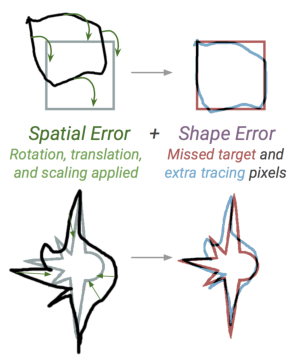
\includegraphics{figs/image-1} 

}

\caption[Measurement of tracing task performance reflects both spatial and shape error components]{Measurement of tracing task performance reflects both spatial and shape error components. Left: The grey shape is the target; the black shape is the raw tracing. After applying affine image registration, the spatial error reflects the extent of translation, rotation and scaling transformation required to minimize shape error. Right: Shape error reflects how closely the contour of the transformed tracing aligns with the target.}\label{fig:image}
\end{figure}
\end{CodeChunk}

\subsection{Visual feature analysis}\label{visual-feature-analysis}

\subsubsection{Deep Convolutional Neural Network
Model}\label{deep-convolutional-neural-network-model}

We used a standard, pre-trained implementation of the VGG-19
architecture (Simonyan \& Zisserman, 2014) to extract features from
sketches at the last full-connected layer of the network known to
support category recognition in both photos and sketches of object
categories. Each image elicits a pattern of feature activations in a
given layer; here, we extract features from the last layer of VGG-19
(Layer 7), known to be an appropriate basis for inferring category
membership (Kubilius et al., 2016) resulting in 4096 features per image
(as fixed by VGG-19). All features were normalized across the entire set
of drawings before analysis.

\subsubsection{Logistic Regression
Classifier}\label{logistic-regression-classifier}

First, in order to create a balanced classification dataset, the dataset
was randomly under sampled such that there were an equal number images
for each of the 23 categories (N=8695 drawings total). To estimate the
recognizability of drawings produced by children in each age group,
model features (see above) were then used to train a 23-way logistic
regression model (as there were 23 possible categories) with L2
regularization under leave-one-out cross-validation. This iterative
modeling procedure yielded a both a binary classification score for each
image as well as the probability that each image was assigned to each
category in the dataset.

\subsubsection{Model Fitting}\label{model-fitting}

We anticipated that classification performance might vary along
dimensions directly related to the motor production demands of the task,
such as the amount of time spent drawing, the number of strokes used,
and amount of ink used (i.e., mean pixel intensity of sketch). In order
to assess whether children's ability to produce recognizable drawings
increased with age, independent of these covariates, we fit a
generalized linear mixed-effects model predicting classification
accuracy. This models included as predictors: children's average tracing
score, scaled age (in years), drawing duration (in seconds), amount of
ink used, and number of strokes as fixed effects, and with random
intercepts for each individual child and object category. To assess
whether children's ability to produce more typical drawings increased
with age, we restricted our analysis to correctly classified drawings
and examined the factors that predicted the probability assigned to the
target category (i.e., classification `confidence').

\subsubsection{Distinctiveness Analyses}\label{distinctiveness-analyses}

We evaluated how distinct different category clusters were at each age
by calculating changes in a high-dimensional analogue of d-prime
(distinctiveness). This metric computes how distinct two category
representations (e.g., bird, rabbit) are by accounting for both the
relative distances between two categories as well as their relative
overlap. For each pair of categories, we first computed the mean feature
vector, which allows an estimate of the category center. To assess the
dispersion of each category, we computed the root-mean-squared deviation
of drawings from this category center using euclidean distance. Using
these two metrics, we can then compute this sensitivity measure by
taking the euclidean distance between any two category centers and
dividing it by the square root of half of the sum of the two category
dispersions. Formally, this is specified as:
\[D(d)_{ij} = \frac{\sqrt{\sum_{i=1}^n (\vec{r}_{i}-\vec{r}_{j})^2}} {\sqrt{1/2 * (CD_{i}^2 + CD_{j}^2})},\]
where \(\vec{r}_{i}\) and \(\vec{r}_{j}\) are the mean feature vectors
for the \(i\)th and \(j\)th object categories, respectively, and where
\(CD\) represents the category dispersion, or the root-mean-squared
deviation of each category, and where D represents the distinctiveness
of two categories. This metric was computed for each pair of categories
within each age group (see Figure 6).

We also separately examined changes in relative distances between
categories following Kriegeskorte, Mur, \& Bandettini (2008). To do so,
we took the Pearson correlation distances between all category centers
(Kriegeskorte et al., 2008) to construct 23x23 representational
dissimilarity matrices (RDM); these RDMs provide a compact description
of the layout of these categories in this high-dimensional feature
space. To assess changes in this representational layout across age, we
computed the Spearman rank correlations between the RDMs between at each
age vs.~the oldest children in our sample (10-year-olds)

\begin{CodeChunk}
\begin{figure*}[h]

{\centering 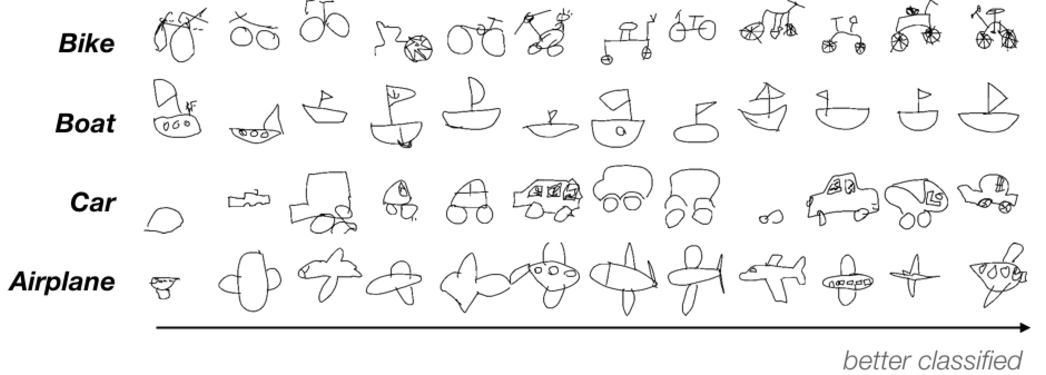
\includegraphics{figs/drawingExamples-1} 

}

\caption[Randomly sampled drawings from eight categories ordered by the probability that the sketch was assigned to the correct target category]{Randomly sampled drawings from eight categories ordered by the probability that the sketch was assigned to the correct target category. All sketches depicted here were correctly classified.}\label{fig:drawingExamples}
\end{figure*}
\end{CodeChunk}

\begin{CodeChunk}
\begin{figure*}[h]
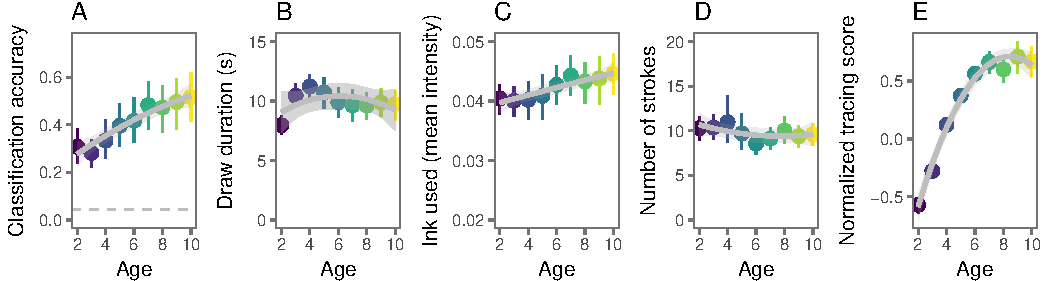
\includegraphics{figs/mainResults-1} \caption[ Leave-one-out classification accuracy (A), the amount of time spent drawing in seconds (B), the amount of ink used (i.e., mean intensity of the drawings) (C), ad the number of strokes used (D) and the (E) average normalized tracing scores are plotted as a function of children’s age]{ Leave-one-out classification accuracy (A), the amount of time spent drawing in seconds (B), the amount of ink used (i.e., mean intensity of the drawings) (C), ad the number of strokes used (D) and the (E) average normalized tracing scores are plotted as a function of children’s age.}\label{fig:mainResults}
\end{figure*}
\end{CodeChunk}

\section{Results}\label{results}

\subsection{Model classification
results}\label{model-classification-results}

Overall, drawing classification accuracy increased with age (see Figure
2). Our mixed-effects model on drawing classification revealed that this
age-related gain held when accounting for task covariates --- the amount
of time spent drawing, the number of strokes, and total ink used --- and
for variation across object categories and individual children. All
model coefficients can be found in Table 1.

We found the same pattern of results when when restricting our analyses
to drawings that were correctly classified and examining the average
probability assigned to the target category (see Figure 3 for examples
ordered by classification confidence). These results suggest that
developmental changes in these high-level visual features of children's
drawings directly lead to gains in category classification accuracy and
confidence.

\subsection{Contributions of fine-motor
skills}\label{contributions-of-fine-motor-skills}

\begin{CodeChunk}
\begin{figure*}[h]
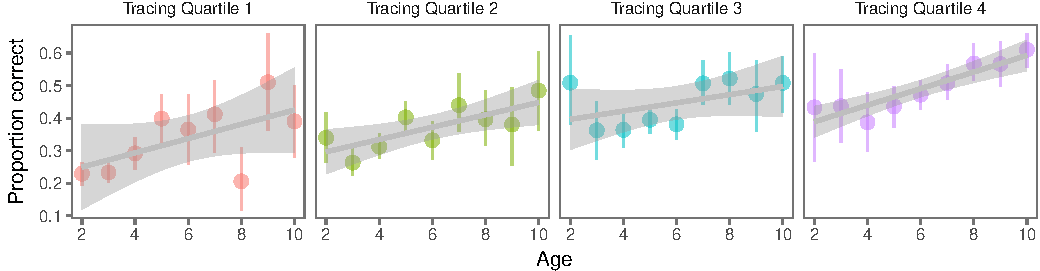
\includegraphics{figs/tracingResults-1} \caption[Data are divided into four quantiles based on the distribution of tracing scores in the entire dataset]{Data are divided into four quantiles based on the distribution of tracing scores in the entire dataset; these divisions represent the data in each panel. In each panel, the average probability assigned to the target class is plotted as a function of child’s age.  Error bars represent 95\% CIs bootstrapped across category means within each age group and subset of tracing scores.}\label{fig:tracingResults}
\end{figure*}
\end{CodeChunk}

\begin{CodeChunk}
\begin{figure*}[h]

{\centering 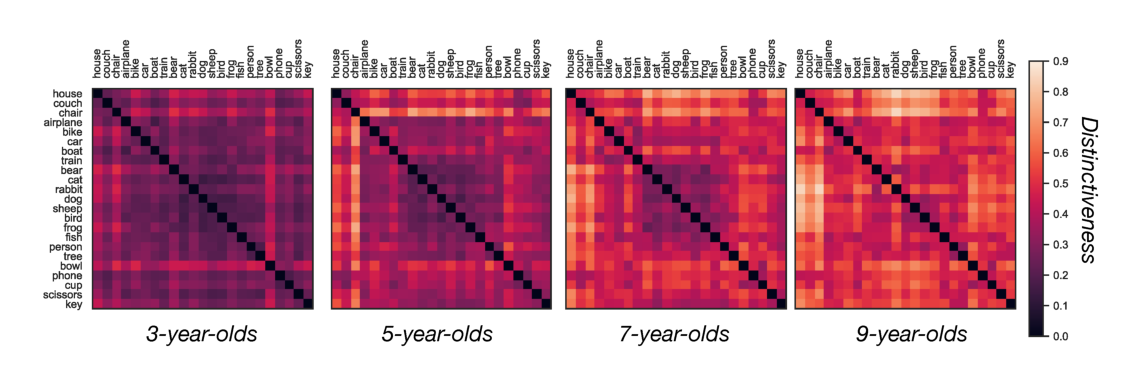
\includegraphics{figs/distinctiveness-1} 

}

\caption[Pairwise category distinctiveness for drawings made by 3-, 5-, 7-,and 9-year-olds]{Pairwise category distinctiveness for drawings made by 3-, 5-, 7-,and 9-year-olds; darker values present pairs of categories that have more overlapping representations; lighter values represent pairs of categories with more distinctive representations.}\label{fig:distinctiveness}
\end{figure*}
\end{CodeChunk}

We next examined the relationship between children's ability to trace
complex shapes and the subsequent recognizability of their drawings
completed at the station. Overall, we found that tracing abilities
increased with age (see Figure 2E) and that individual's tracing
abilities were good predictors of the recognizability of the drawings
they produced (classification accuracy: \(\beta\) = 0.31, SE = 0.035, Z
= 9.1). This main effect of tracing ability also held when accounting
for task covariates (number of strokes, time spent drawing, ink used).
However, we found that children's tracing abilities did not interact
with the age-related gains in classification we observed (see Figure 4):
there was no interaction between age and tracing ability (classification
accuracy: \(\beta\) = -0.07, SE = 0.034, Z = -2.1) and we observed
age-related classification gains at each level of tracing ability.

\subsection{Distinctiveness analyses}\label{distinctiveness-analyses-1}

`

What changes in the feature space might be driving increases in
classification accuracy over development? We hypothesized that these
increases in classification would be paralleled by an increase in the
distinctiveness of the depicted categories in this high-level visual
features. We computed category distinctiveness by evaluating a
higher-dimensional analog of d-prime that accounts for both changes in
the relative distances between category centers as well as their
relative dispersions. Overall, we found an overall increase in the
distinctiveness between object categories with age (see Figure 5). This
increase seemed to be driven by both changes in relative distances
between category centers changed across age as well as changes in
relative dispersions within-categories: the similarity between RDMs for
each age group vs.~10-year-olds increased with age, and category
clusters shrank slightly across age (see Figure 6).

\section{General Discussion}\label{general-discussion}

How do children represent different object categories throughout
childhood? Drawings are a rich potential source of information about how
visual representations change over development. One possibility is that
older children's drawings are more recognizable because the children are
better able to include the distinctive features of particular categories
that set them apart from other similar objects. Supporting this
hypothesis, the high-level visual features present in children's
drawings could be used to estimate the category children were intending
to draw, and these classifications became more accurate as children
became older. These age-related gains in classification were not
explainable by either low-level task covariates (e.g., amount of time
spent drawing, average intensity, or number of strokes) or children's
tracing abilities.

Taken together, these results suggest that children's drawings contain
more distinctive features as they grow older, perhaps reflecting a
change in their internal representations of these categories. However,
one possibility is that children simply learn routines to draw certain
categories---perhaps from direct instruction or observation.
Nonetheless, our results held even when restricted to a subset of very
rarely drawn categories (e.g., ``couch'',''scissors'',''key''),
providing evidence against a simple version idea.

Thus, these results open the door for future work to examine the ways in
which children's drawings are linked to their changing visual concepts.
One possibility is that children's drawing of object categories are
intimately linked to their visual recognition behaviors: children who
produce these more distinctive features in their drawings have
finer-grained perceptual representations of these categories. On this
account, younger children who tend to not draw these features may have
lossier visual representations of these categories, and show poorer
recognition behaviors. A second possibility, however, is that when
children are asked to draw ``a rabbit'' they could also access on a list
of conceptual attributes that they remember that rabbits have (e.g.,
bushy tails, long ears, whiskers). If this is the case, then we might
instead observe a relationship between the features that children list
when asked to describe ``a rabbit'' and the features that children draw.

Overall, we suggest that children's drawings change systematically
across development, and that they contain rich information about
children's underlying representations of the categories in the world
around them. By leveraging this natural behavior, we can quickly and
easily collect large-scale datasets across childhood that allow us to
make detailed inferences about the shape of developmental changes. A
full understanding of how children's drawings reflect their emerging
perceptual and conceptual knowledge will allow a unique and novel
perspective on the both the development and the nature of visual
concepts---the representations that allow us to easily derive meaning
from what we see.

\section{Acknowledgements}\label{acknowledgements}

Place acknowledgments (including funding information) in a section at
the end of the paper.

\section{References}\label{references}

\setlength{\parindent}{-0.1in} \setlength{\leftskip}{0.125in} \noindent

\hypertarget{refs}{}
\hypertarget{ref-arden2014genes}{}
Arden, R., Trzaskowski, M., Garfield, V., \& Plomin, R. (2014). Genes
influence young children's human figure drawings and their association
with intelligence a decade later. \emph{Psychological Science},
\emph{25}(10), 1843--1850.

\hypertarget{ref-barrett1976symbolism}{}
Barrett, M., \& Light, P. (1976). Symbolism and intellectual realism in
children's drawings. \emph{British Journal of Educational Psychology},
\emph{46}(2), 198--202.

\hypertarget{ref-bozeat2003duck}{}
Bozeat, S., Lambon Ralph, M. A., Graham, K. S., Patterson, K., Wilkin,
H., Rowland, J., \ldots{} Hodges, J. R. (2003). A duck with four legs:
Investigating the structure of conceptual knowledge using picture
drawing in semantic dementia. \emph{Cognitive Neuropsychology},
\emph{20}(1), 27--47.

\hypertarget{ref-bremmer1984prior}{}
Bremner, J. G., \& Moore, S. (1984). Prior visual inspection and object
naming: Two factors that enhance hidden feature inclusion in young
children's drawings. \emph{British Journal of Developmental Psychology},
\emph{2}(4), 371--376.

\hypertarget{ref-FanCommon2018}{}
Fan, J. E., Yamins, D. L. K., \& Turk-Browne, N. B. (2018). Common
object representations for visual production and recognition.
\emph{Cognitive Science}, \emph{0}(0).
\url{http://doi.org/10.1111/cogs.12676}

\hypertarget{ref-freeman1987current}{}
Freeman, N. H. (1987). Current problems in the development of
representational picture-production. \emph{Archives de Psychologie}.

\hypertarget{ref-fury1997children}{}
Fury, G., Carlson, E. A., \& Sroufe, A. (1997). Children's
representations of attachment relationships in family drawings.
\emph{Child Development}, \emph{68}(6), 1154--1164.

\hypertarget{ref-juttner2016developmental}{}
Juttner, M., Wakui, E., Petters, D., \& Davidoff, J. (2016).
Developmental commonalities between object and face recognition in
adolescence. \emph{Frontiers in Psychology}, \emph{7}.

\hypertarget{ref-karmiloff1990constraints}{}
Karmiloff-Smith, A. (1990). Constraints on representational change:
Evidence from children's drawing. \emph{Cognition}, \emph{34}(1),
57--83.

\hypertarget{ref-kellogg1969analyzing}{}
Kellogg, R. (1969). \emph{Analyzing children's art}. National Press
Books Palo Alto, CA.

\hypertarget{ref-kriegeskorte2008RSA}{}
Kriegeskorte, N., Mur, M., \& Bandettini, P. (2008). Representational
similarity analysis--connecting the branches of systems neuroscience.
\emph{Frontiers in Systems Neuroscience}, \emph{2}.

\hypertarget{ref-kubilius2016deep}{}
Kubilius, J., Bracci, S., \& Op de Beeck, H. P. (2016). Deep neural
networks as a computational model for human shape sensitivity.
\emph{PLoS Computational Biology}, \emph{12}(4), e1004896.

\hypertarget{ref-long2018drawings}{}
Long, B., Fan, J., \& Frank, M. (2018). Drawings as a window into the
development of object category representations. \emph{Journal of
Vision}, \emph{18}(10), 398--398.

\hypertarget{ref-mash2006}{}
Mash, C. (2006). Multidimensional shape similarity in the development of
visual object classification. \emph{Journal of Experimental Child
Psychology}, \emph{95}(2), 128--152.

\hypertarget{ref-minsky1972artificial}{}
Minsky, M., \& Papert, S. A. (1972). Artificial intelligence progress
report.

\hypertarget{ref-nishimura2009}{}
Nishimura, M., Scherf, S., \& Behrmann, M. (2009). Development of object
recognition in humans. \emph{F1000 Biology Reports}, \emph{1}.

\hypertarget{ref-piaget1929child}{}
Piaget, J. (1929). The child's concept of the world. \emph{Londres,
Routldge \& Kegan Paul}.

\hypertarget{ref-rehrig2018does}{}
Rehrig, G., \& Stromswold, K. (2018). What does the dap: IQ measure?:
Drawing comparisons between drawing performance and developmental
assessments. \emph{The Journal of Genetic Psychology}, \emph{179}(1),
9--18.

\hypertarget{ref-sandkuhler2018}{}
Sandkühler, R., Jud, C., Andermatt, S., \& Cattin, P. C. (2018). AirLab:
Autograd image registration laboratory. \emph{ArXiv Preprint
ArXiv:1806.09907}.

\hypertarget{ref-simonyan2014very}{}
Simonyan, K., \& Zisserman, A. (2014). Very deep convolutional networks
for large-scale image recognition. \emph{ArXiv Preprint
ArXiv:1409.1556}.

\hypertarget{ref-yamins2014performance}{}
Yamins, D., Hong, H., Cadieu, C. F., Solomon, E. A., Seibert, D., \&
DiCarlo, J. J. (2014). Performance-optimized hierarchical models predict
neural responses in higher visual cortex. \emph{Proceedings of the
National Academy of Sciences}, \emph{111}(23), 8619--8624.

\bibliographystyle{apacite}


\end{document}
